\chapter{Experiments and Results}
\label{chap:ExperimentsAndResults}

This chapter begins with a detailed description of the training process. Follows an in-depth exploration, discussion and experimentation regarding major hyperparameters, where each section concludes with the choice of a default value for that parameter. Finally, each of the last three sections presents an experiment we performed:

\begin{itemize}
    \item Measure the impact of adding different amounts of unsupervised data during training (Section \ref{sec:SemisupervisedImprovements}).
    \item Measure the impact of model size (number of synapses) on the task performance, when training on all available handwritten data (Section \ref{sec:UtilizingCvcMuscima}).
    \item Attempt to learn the segmentation task on printed music and evaluate it on handwritten music, while using unlabeled handwritten music as regularization (Section \ref{sec:KnowledgeTransfer}).
\end{itemize}


\section{Training}
\label{sec:Training}

There are many ways in which a semi-supervised generative model can be trained. One option is to pre-train a model in the unsupervised mode and after that train a separate supervised part of the model (\cite{KingmaSslVae}). Another option is to run the supervised training as a fine-tuning step after the unsupervised training, similar to the transfer learning approach. We chose to train both the supervised and the unsupervised tasks simultaneously, using a single, composite loss function.

One training step has the following structure:

\begin{itemize}
    \item An input image is passed through the network and the produced segmentation is compared to the gold one, producing the supervised loss.
    \item An input image with noise added is passed through the network and the produced reconstruction is compared to the clean input image, producing the reconstruction loss.
    \item The reconstruction loss is multiplied by a constant hyperparameter we call \emph{unsupervised loss weight}. Both losses are summed to produce the composite loss.
    \item The composite loss is used to calculate model gradients.
    \item An optimizer uses these gradients to update model weights.
\end{itemize}

The input to the training step is a composite batch of $(x_l, y_l)$ labeled data pairs and $(x_u, y_u)$ unlabeled data pairs.

\begin{itemize}
    \item $x_l$ are input images for segmentation
    \item $y_l$ are gold segmentation masks
    \item $x_u$ are noised input images for reconstruction
    \item $y_u$ are cleaned target reconstruction images
\end{itemize}

The number of labeled and unlabeled pairs in a composite batch differs and their ratio is related to the ratio of labeled to unlabeled data in the dataset. The hyperparameter \emph{batch size} dictates the total number of labeled and unlabeled pairs in one composite batch.

\begin{figure}[ht]
    \centering
    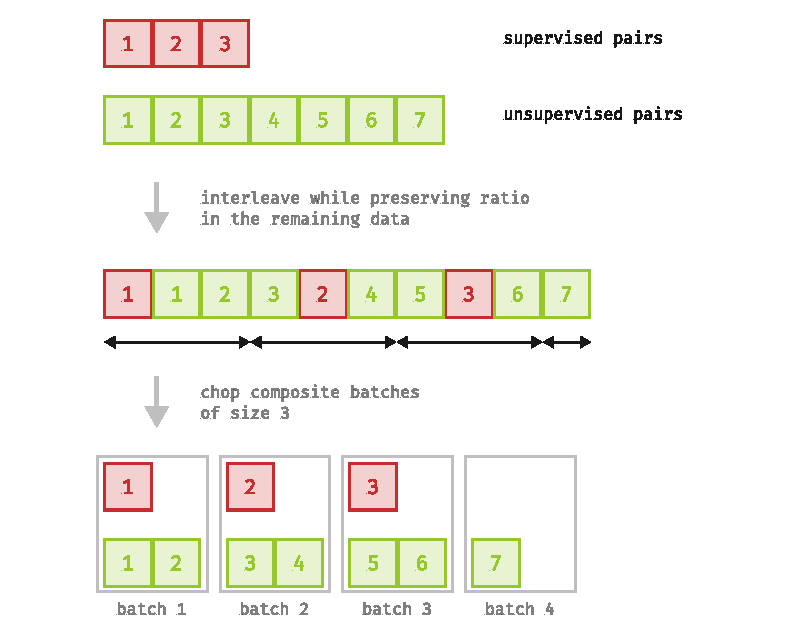
\includegraphics[width=140mm]{../img/batching-process.pdf}
    \caption{Illustration of how are supervised and unsupervised training pairs combined to form composite training batches.}
    \label{fig:CompositeBatching}
\end{figure}

Composite batches are created by taking training pairs from the labeled and unlabeled splits of the dataset. When the next pair is taken, we either take it from the labeled or the unlabeled split, whichever is larger, with respect to their target ratio. For example, if their ratio in the whole dataset is 1:5 (labeled to unlabeled) and we have 10:201 remaining pairs, we will take an unlabeled pair next. We take pairs until we have \emph{batch size} number of them and then we send them to the training logic as a new composite batch.

To be able to batch together the training images, they need to have the same spatial dimensions. For this reason we do not train on the entire music pages, but instead on tiles of fixed size. The size is set to 512 pixels wide and 256 pixels high for all experiments. We took inspiration for this from the article by \cite{HajicEtAl}. Tiles are sampled from a music page at random locations and the number of tiles is equal to the area of the page, divided by the area of the tile. The article also employs a technique called oversampling, where a tile is sampled up to five times if it contains no pixel of the target segmentation class. This technique helps with training on rare symbols (e.g. clefs), where most tiles would contain no instance of the target class. Our training logic also implements this oversampling technique.

The semantic segmentation task is usually framed as a pixelwise classification problem. For this reason we use the pixelwise binary crossentropy loss function (\cite{DeepLearningBook}). To make the loss value invariant to changes in \emph{batch size} and \emph{tile size}, we compute the average over all pixels in a batch. This allows us to sum the supervised and unsupervised losses, as they are of a similar magnitude, regardles of the number of labeled and unlabeled training pairs used. The reconstruction task will also use the same pixelwise binary crossentropy loss function, since the reconstruction of a single pixel can be understood as the probability of that pixel being black.

We use the Adam optimizer for all experiments, with learning rate $0.001$, $\beta_1 = 0.9$, $\beta_2 = 0.999$ and $\varepsilon = 10^{-7}$ (\cite{AdamOptimizer}). Also, for all experiments, we use the validation dataset to assess the performance of the model and train for as long as it is improving. Any evaluation of any trained model is performed by the model with the optimal validation dataset performance (unless the entire validation training curve is shown).


\section{Understanding Hyperparameters}
\label{sec:UnderstandingHyperparameters}


\subsection{Batch Size}
\label{sec:BatchSize}

In the deep learning field, it is known that having a small batch size makes the training fast and noisy, whereas a large batch size makes it more stable at the cost of being slower (\cite{DeepLearningBook}). Since our model is fully convolutional and we train it on image tiles of fixed size, we can consider the size of these tiles to be a parameter similar to batch size. It also regulates the amount of data used for gradient estimation. If these tiles are large enough, we can get away with batch size of 1 (this is what the original U-Net article does (\cite{UNet})).

Using such a small batch size is, however, not possible in our case. Our training process expects batches containing both labeled and unlabeled data. Batch size determines the total number of these two kinds of data items in the entire composite batch. The ratio of these two item types within the composite batch is dictated by the ratio within the whole dataset. So if our dataset has, for example, 1:5 labeled to unlabeled data, the batch size has to be at least 6. Otherwise we will start getting batches that contain only unlabeled data. This rule is not as strict, since the model would probably learn both tasks even if half of all batches were missing labeled data, however, if the imbalance becomes too severe, the training fails.

\begin{figure}[ht]
    \centering
    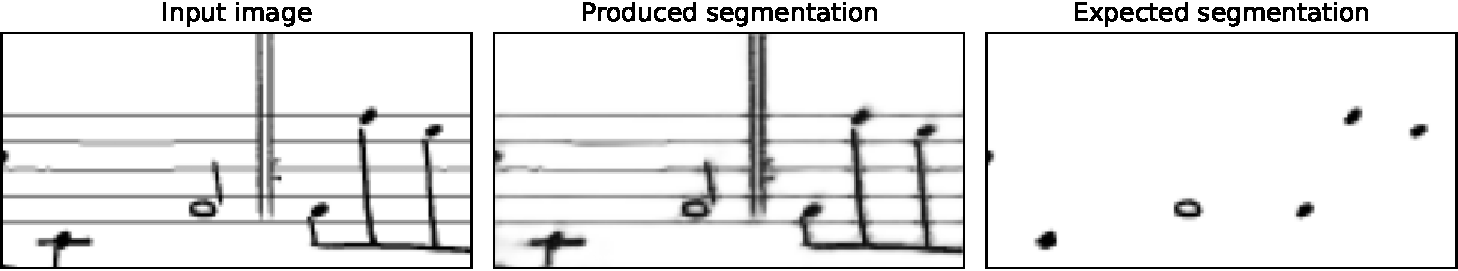
\includegraphics[width=140mm]{../../figures/07-small-batches/small-batches.pdf}
    \caption{When batches are too small, some of them will lack labeled data and the model will fail to learn the supervised segmentation task. Instead, reconstruction output leaks into the segmentation output. This example has batch size 2 and 1:10 ratio.}
    \label{fig:SmallBatches}
\end{figure}

An example of such a failing training can be seen in figure \ref{fig:SmallBatches}. The model learns to perform reconstruction even for the segmentation task. This is understandable, since the two tasks are differentiated only at the last layer (1x1 sigmoid convolution). If all second-to-last layer activations contain image reconstruction data, then any 1x1 convolution combination of them will do as well.

Since all of our experiments have training data ratios between 1:0 and 1:10, we chose to set the batch size parameter to 10.


\subsection{Dropout}
\label{sec:Dropout}

The network architecture, as described in section \ref{sec:Architecture}, contains a dropout layer within every convolutional block (\cite{Dropout}). We use the dropout when training on small datasets (experiment \ref{sec:SemisupervisedImprovements}), because the training is otherwise very noisy and it is difficult to infer any measurable differences between runs. We use dropout as a mean to stabilize the training, which in this setting also slightly increases model accuracy.

When training on larger datasets, the training is no longer unstable and dropout is not needed (experiments \ref{sec:UtilizingCvcMuscima} and \ref{sec:KnowledgeTransfer}). In fact, it causes the training process to converge much slower (2x or more) and it does not increase model accuracy anymore.

Both the original U-Net article (\cite{UNet}) and the article by \cite{HajicEtAl} use the U-Net architecture without any dropout. In fact, an article by \cite{DropoutOnConvolutions} argues, that using traditional dropout on convolutional layers may not be ideal. This agrees with our findings, that dropout helps only in very specific circumstances.

It may be the case, that using batch normalization instead or dropout (like \cite{HajicEtAl}) has the same effect of regularizing the network. However our goal is not to find the optimal architecture, but to measure the impact of unsupervised data. For that reason we did not explore this option further.

From all this we conclude that dropout should be disabled by default.


\subsection{Skip Connections}
\label{sec:SkipConnections}

In the chapter about our architecture (\ref{sec:Architecture}) we described a method for disabling skip connections during reconstruction training. We present three modes for skip connections:

\begin{itemize}
    \item solid -- skip connections are always enabled, like in a typical U-Net archtiecture
    \item gated -- skip connections are enabled for the supervised task (traitraining and inference) and disabled for the reconstruction task (training and inference)
    \item none -- skip connections are always disabled, like in a typical autoencoder
\end{itemize}

The motivation behind gating skip connections is to bring the U-Net architecture (\cite{UNet}) closer to a more traditional fully-convolutional autoencoder archtiecture (\cite{AutoencodersOverview}).

To measure the effect of skip connections, we propose the following experiment. We take the 16 \emph{inner feature}, semi-supervised model from experiment \ref{sec:UtilizingCvcMuscima} and train it with various skip connection settings. Training curves are shown in figure \ref{fig:SkipConnections}.

\begin{figure}[ht]
    \centering
    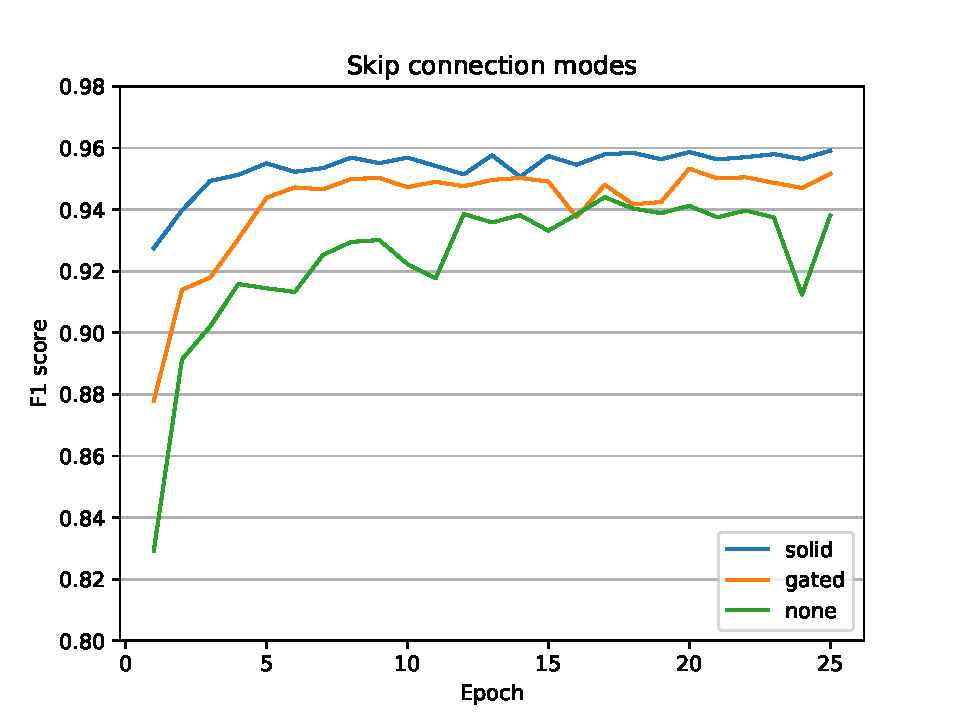
\includegraphics[width=140mm]{../../figures/05-skip-connections/skip.pdf}
    \caption{Comparing various skip connection modes with a model from experiment \ref{sec:UtilizingCvcMuscima} (16 inner features, semi-supervised). The permanent skip connection mode performs the best, although all runs are below the supervised baseline. The order could be different, should the baseline be exceeded.}
    \label{fig:SkipConnections}
\end{figure}

We can see that solid and gated modes have the best performance. The model with no skip connections is clearly worse at the segmentation task. This result validates the superiority of the U-Net architecture for semantic segmentation.

The gated mode seems to perform worse than the solid one. Despite this, we chose to train all the experiments in this gated mode as we belive it helps the model to learn representations during unsupervised training.

We have to point out, that all of our semi-supervised experiments never exceeded their supervised baselines. This means that bringing the model closer to its supervised setting (using solid skip connections) should increase its performance, because we are bringing it closer to the baseline. For this reason we cannot conclude, what the best skip connection mode would be, if we managed to exceed the baseline. It is possible the order of modes would get reversed. This is another reason why we chose to use gated connections, despite not being optimal in this experiment.


\subsection{Unsupervised Loss Weight}
\label{sec:UnsupervisedLossWeight}

This parameter determines the relative magnitude of the segmentation and the reconstruction loss. We first thought this parameter would have significant impact on the training and would need to be tuned carefully. It turned out not to be the case. We ended up setting it 1 and not optimizing it.

Varying this parameter from 10 to 0.1 has minimal impact on model performance. When we examined infered segmentation masks and reconstructed images, as they evolve throughout the training process, we discovered that this parameter primarily impacts the speed at which the two tasks are learned relative to each other. When the parameter is 10, the reconstruction task is learned quickly and segmentation task is learned slowly. When we set it 0.1 the situation is reversed. If we let the training converge, it ends up learning both tasks equally well.

Interesting behaviour happens only at the extreme. When the parameter is set to zero, the reconstruction task produces no gradients and the training collapses to the fully-supervised regime. We performed an experiment that verified this behaviour.


\subsection{Noise Parameters}
\label{sec:NoiseParameters}

\begin{figure}[p]
    \centering
    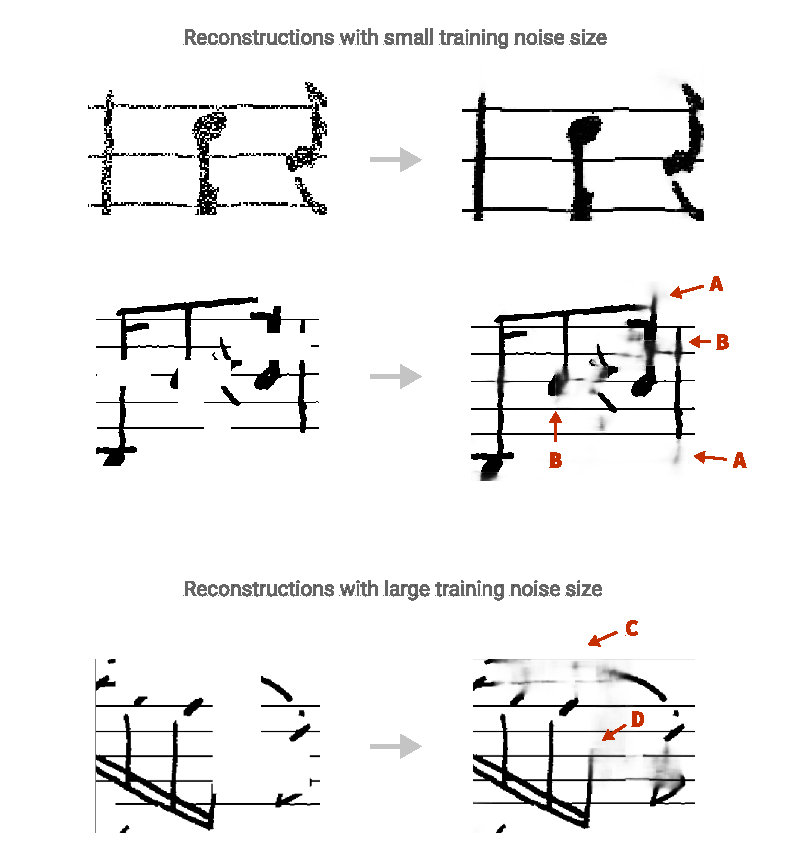
\includegraphics[width=140mm]{../../figures/06-noise/noise-size.pdf}
    \caption{Comparing reconstructions performed by models trained with small and large noise tiles. (A) Low-level reconstructions, make no sense in the musical context. (B) Edges of dropped tiles leaking into the reconstruction. (C) High-level reconstruction with staffliens and stems visible. (D) Forgotten notehead.}
    \label{fig:NoiseSize}
\end{figure}

There are two major nosie parameters that can be varied:

\begin{itemize}
    \item Noise resolution (size of dropout squares)
    \item Noise dropout ratio (ratio of erased input pixels)
\end{itemize}

In the section on noise generation (\ref{sec:NoiseGeneration}) we gave reasons for using larger noise resolution (but not too large). We belive large tiles force the model to learn larger symbols and thus the corresponding high-level representations. This hypothesis is supported by images shown in the figure \ref{fig:NoiseSize}.

The first two images show, how the model learns to remove small noise easily. The model, however, does not produce satisfying reconstructions when applied to an image with larger noise tiles dropped (as seen in the second pair of images). We can see that:

\begin{itemize}
    \item Edges of noise tiles are still visible in the reconstruction.
    \item Reconstructed stafflines fade when they are close to other symbols.
    \item Most reconstructions are based on relatively low-level features. The beam corner is extended upwards, which is reasonable in the sense of drawing straight lines, but not in any musical sense.
\end{itemize}

Comparatively, the lower two images show a much better reconstruction. The lower reconstruction was trained with noise size equal to the size seen in the lower left image. Reconstructed stafflines are sharp even when intersecting the eighth note and there are no tile edges visible (reconstructions blend well with the known image). The model has even managed to conjure up a fake set of stafflines and stems, that connect well to visible noteheads (pointer C). This shows that the model learns much higher-level features than just simple geometric shapes (lines, circles).

We ended up training all experiments with noise tiles of size equal to two staff spaces and noise dropout ratio of 25\%. We experimented with noise dropout of 50\%, but the performance seemed not to change. This chosen size and ratio can be seen in the last row of figure \ref{fig:NoiseSize}.


\subsection{Activation Function}
\label{sec:ActivationFunction}

We first used ReLU activation function (rectified linear unit) in all convolutional layers (except the final sigmoid layer), just like it is used in the original U-Net article (\cite{UNet}). However, we occasionally encountered problems with convergence. Replacing the activation function with ELU (exponential linear unit) solved these issues. We took inspiration from \cite{DorferEtAl}, who also use the ELU activation function. The difference between the two can be seen in figure \ref{fig:ActivationFunctions}.

\begin{figure}[ht]
    \centering
    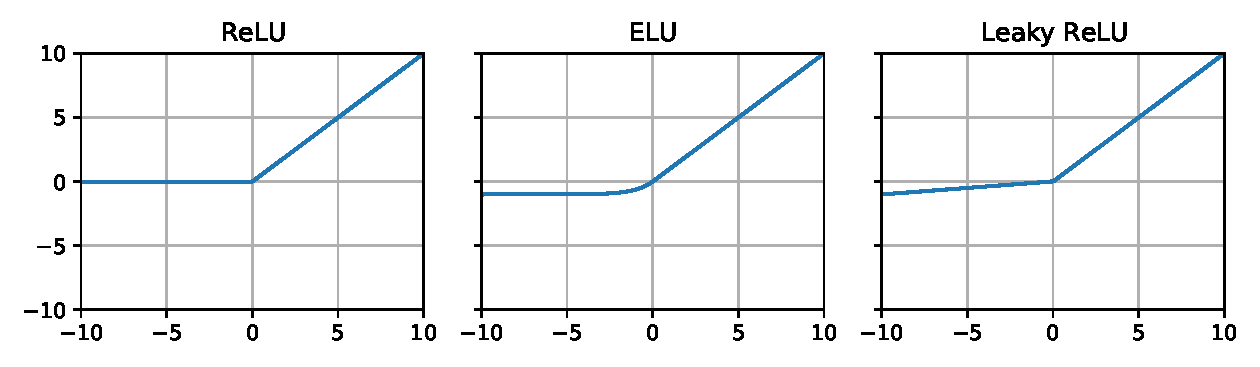
\includegraphics[width=140mm]{../../figures/03-activation-function/functions.pdf}
    \caption{Visualization of explored activation functions. ReLU is flat in negative values and therefore has no gradient there. ELU has exponentially decaying gradient and leaky ReLU has a constant gradient. The parameter for the displayed leaky ReLU is 0.1 to make its shape more apparent.}
    \label{fig:ActivationFunctions}
\end{figure}

The convergence problems were happening at the very beginning of training. The model quickly learned to output a completely black image and never recovered from that state. We think it was an instance of the "dying ReLU" problem (\cite{DyingRelu}). When the model is first initialized, it outputs a gray-ish image, since model weights are drawn from a uniform distribution centered on zero and the final sigmoid layer turns that into a 0.5 gray. Because our target images have black background, the model first learns to produce mostly black images. Only then does it learn to output white pixels as well (see figure \ref{fig:ActivationTrainingProgression}). With ReLU, the first training phase probably overshoots into the negative range of most synapses and that causes the model to get stuck in that negative range with zero gradient.

\begin{figure}[ht]
    \centering
    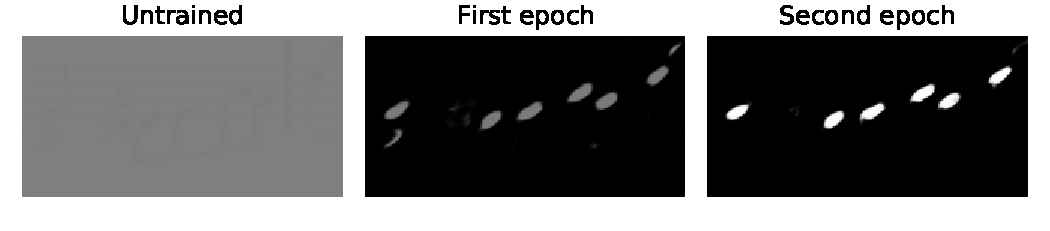
\includegraphics[width=140mm]{../../figures/03-activation-function/progression.pdf}
    \caption{The training process starts by learning to output a mostly black image, which probably causes the model to overshoot during the fully-supervised training and get stuck in the "dying ReLU" problem.}
    \label{fig:ActivationTrainingProgression}
\end{figure}

Interestingly enough, this problem happens only when training in the fully-supervised mode. We have never encountered it, when training in the semi-supervised mode. This again suggests that unlabeled data act as regularization, damping any extreme gradients, and stabilizing the training.

We also tried using the leaky ReLU function with parameter $\alpha = 0.01$, however the problem still remained. Maybe a larger value for $\alpha$ would help, although we already knew that ELU works, so we haven't explored this further.

\begin{figure}[ht]
    \centering
    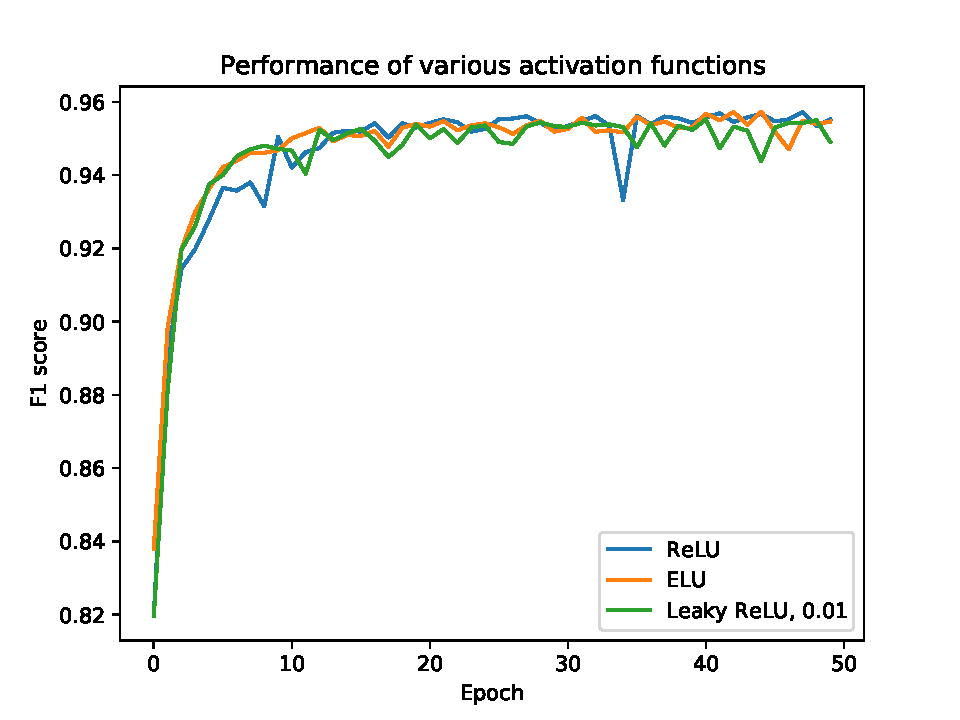
\includegraphics[width=140mm]{../../figures/03-activation-function/performance.pdf}
    \caption{An experiment from section \ref{sec:UtilizingCvcMuscima} with 8 inner features, trained in fully-supervised mode with various activation functions. All runs show the same performance.}
    \label{fig:ActivationFunctionPerformances}
\end{figure}

We run one of the experiments from section \ref{sec:UtilizingCvcMuscima} with all proposed activation functions to see what impact it has on model performance (figure \ref{fig:ActivationFunctionPerformances}). We can clearly see that they all perform equally well, so we choose ELU as the only activation function that does not suffer from the convergence problem. We thereby validate the work of \cite{DorferEtAl} (their article does not provide explanation for the use of ELU, but we belive they must have encountered these exact same problems).


\section{Semi-supervised Improvements}
\label{sec:SemisupervisedImprovements}

The main hypothesis this work is attempting to validate is that adding unlabeled data to the training process helps. We primarily want to improve model accuracy, but as we will see, this is not what our experiments suggest. They do, however, show improvements in other areas, such as training stability and reduced overfitting (section \ref{sec:UtilizingCvcMuscima}).

In this first experiment, we test how various labeled to unlabeled data ratios affect the training process. The experiment uses the MUSCIMA++ dataset (\cite{MuscimaPP}):

\begin{itemize}
    \item 10 pages act as the labeled set.
    \item 0, 5, 10 and 50 pages act as the unlabeled set.
    \item 10 pages act as the validation set.
    \item All of these pages come from the writer-independent train set of MUSCIMA++ and are chosen in a writer-independent manner (all the splits contain pages by different writers).
\end{itemize}

The learned task is notehead segmentation (both full and empty noteheads). Noteheads are an ideal symbol for this kind of measurement. Firstly, they are very abundant. Each page of the dataset contains many instances of them and they are evenly scattered over the whole page. If we were to instead detect more rare symbols (such as clefs or rests), it could skew the results, making it difficult to separate the effects we want to measure. Handwritten noteheads are also very diverse in style, making them more interesting to learn (compared to, say, stafflines).

\begin{figure}[ht]
    \centering
    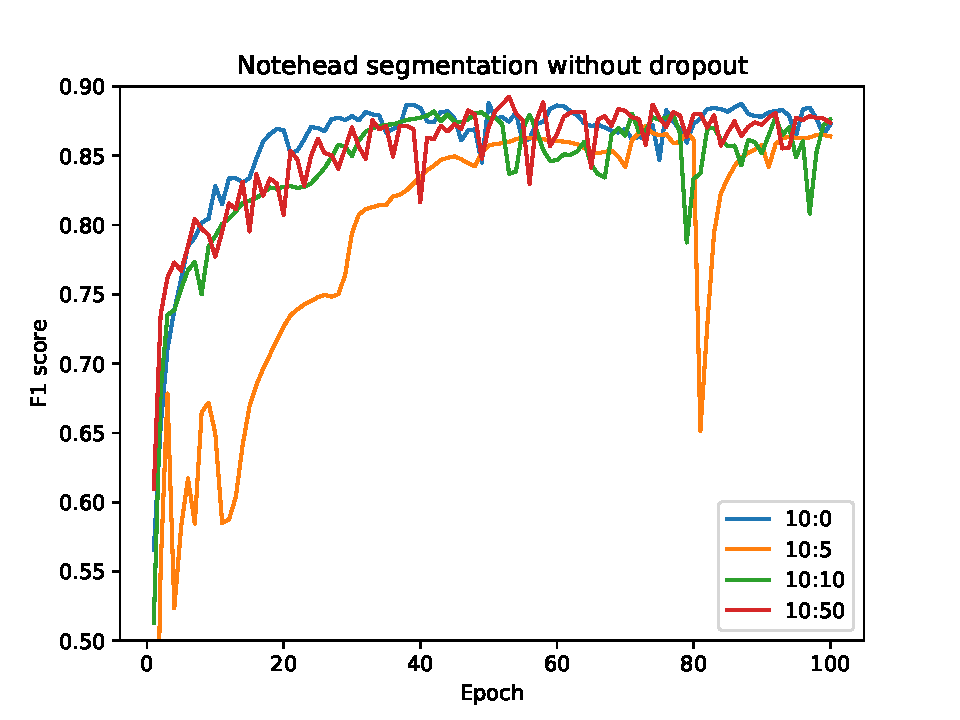
\includegraphics[width=140mm]{../../figures/01-exploration-noteheads/noteheads.pdf}
    \caption{Training on a small dataset without dropout is noisy, see the orange line at the beginning and the green line at the end.}
    \label{fig:ExplorationNoteheadsNoDropout}
\end{figure}

All model hyperparameters are set to sensible deafults. The derivation of these values has been described in section \ref{sec:UnderstandingHyperparameters}. The model capacity, described by the \emph{inner features} parameter is set to 8, which is useful to know for comparison with the next experiment. The proposed dataset is rather small and so the training is very noisy (figure \ref{fig:ExplorationNoteheadsNoDropout}). To stabilize the trainig we set the dropout parameter to 50\% (\cite{Dropout}).

\begin{figure}[p]
    \centering
    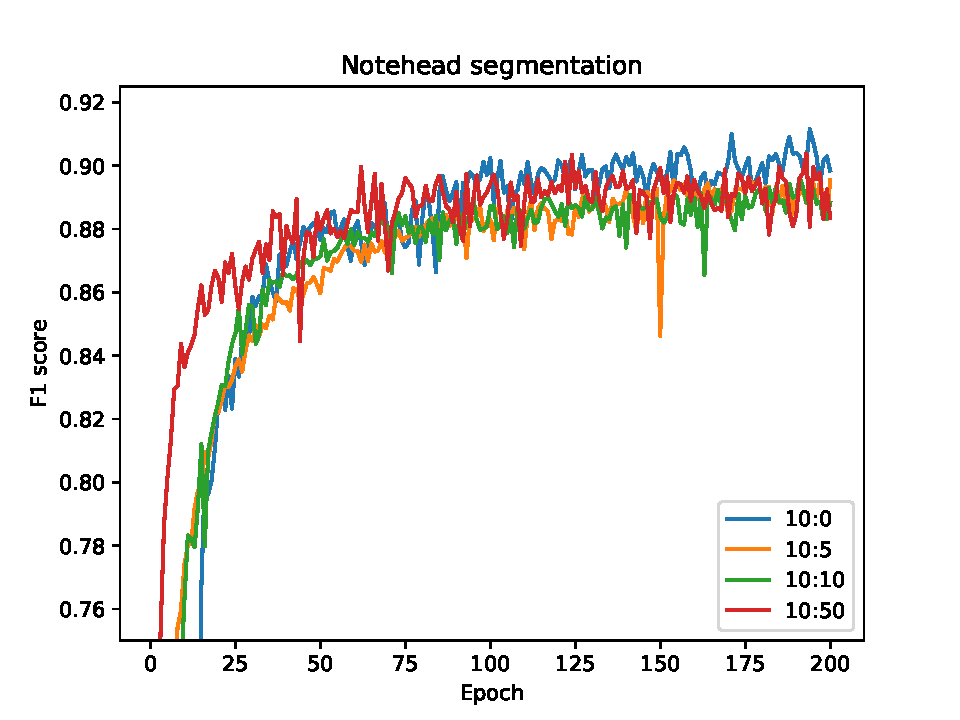
\includegraphics[width=140mm]{../../figures/01-exploration-noteheads/noteheads-dropout.pdf}
    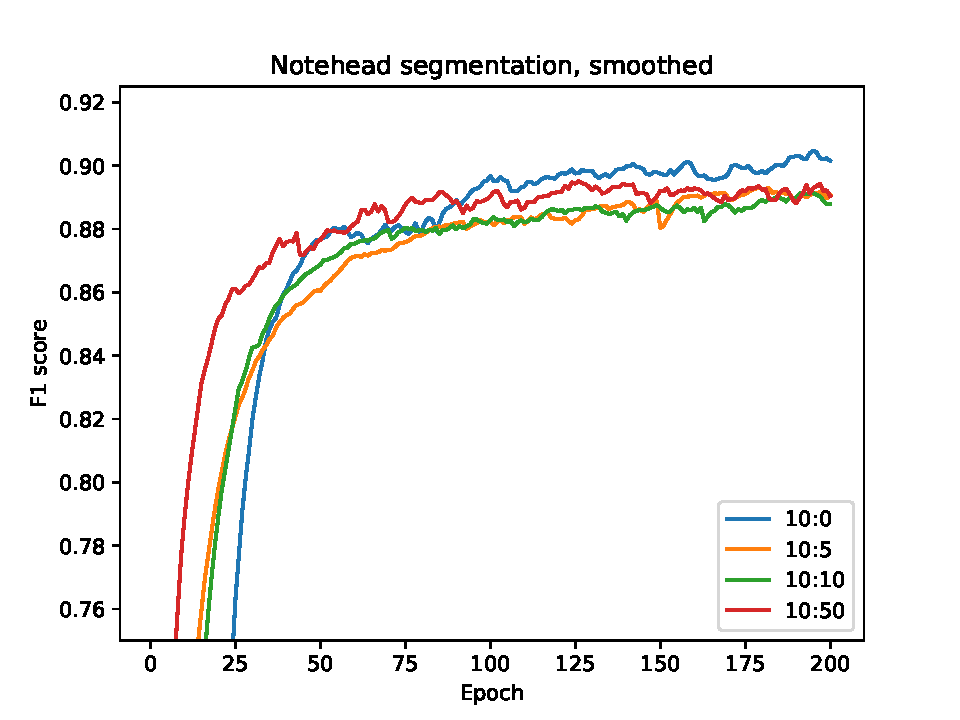
\includegraphics[width=140mm]{../../figures/01-exploration-noteheads/noteheads-dropout-smooth.pdf}
    \caption{Training curves of semi-supervised models with different ratios of supervised and unsupervised data. The bottom image is smoothed using exponential moving average. The fully-supervised baseline (blue) clearly outperforms all semi-supervised models.}
    \label{fig:ExplorationNoteheads}
\end{figure}

We expect that as we add more and more unlabeled data, the F1 score should reach higher and higher. Or at least not get worse. This is not what we see in the figure \ref{fig:ExplorationNoteheads}. The fully supervised model outperforms all the others by a clear margin.

Focusing only on the semi-supervised models, it seems that adding more unsupervised data maybe helps here, although the three lines end up on top of each other at the epoch 200. A better idea is to look at the figure \ref{fig:ExplorationNoteheadsEvaluation}. The chart contains evaluation results on the test set of six runs of each configuration. We can clearly see how the performance rises with more unsupervised data. Unfortunately it does not reach above the fully-supervised results. We unfortunately cannot push the amount of unlabeled data much higher, as it would break our training process (see section \ref{sec:BatchSize}) and it would likely also have diminishing returns. The actual numbers are summarized in table \ref{tab:ExplorationNoteheads}.

The reason for this drop in performance is probably caused by the fact, that the supervised model has to only learn one task -- segmentation. Whereas the semi-supervised one has to also learn the unsupervised reconstruction task. This claim is explored in the next section and is supported by the fact that the performance drop disappears when we increase model capacity.

\begin{figure}[ht]
    \centering
    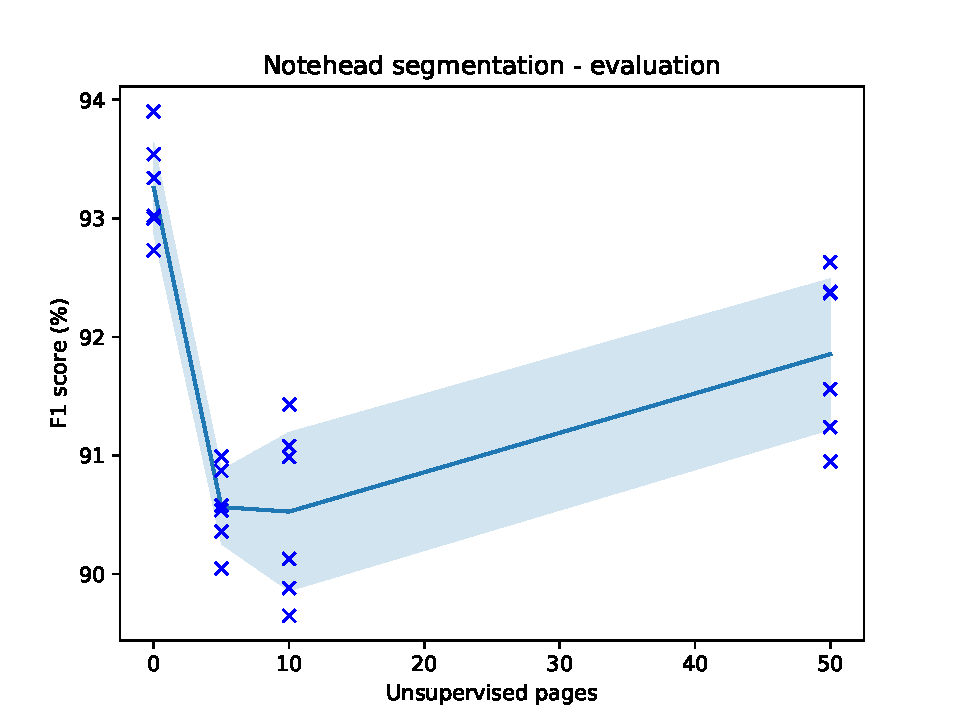
\includegraphics[width=140mm]{../../figures/01-exploration-noteheads/noteheads-evaluation.pdf}
    \caption{Notehead segmentation performance on the MUSCIMA++ writer-independent test set, when trainig with 10 labeled pages and a variable number of unlabeled pages. Adding more unlabeled data helps, but never outperforms the fully-supervised baseline.}
    \label{fig:ExplorationNoteheadsEvaluation}
\end{figure}

\begin{table}[ht]
    \centering
    \begin{tabular}{l@{\hspace{2.0cm}}rrrr}
        \toprule
        \textbf{Page type} & \multicolumn{4}{c}{\textbf{Page count}} \\
        \midrule
        Labeled   & 10 & 10 & 10 & 10 \\
        Unlabeled & 0  & 5  & 10 & 50 \\
        \midrule
        \textbf{Seed} & \multicolumn{4}{c}{\textbf{F1 Score (\%)}} \\
        \midrule
        0 & 92.73 & 90.87 & 91.08 & 92.38 \\
        1 & 93.02 & 90.36 & 90.13 & 91.24 \\
        2 & 93.54 & 90.05 & 89.88 & 91.56 \\
        3 & 93.34 & 90.99 & 89.65 & 92.63 \\
        4 & 93.90 & 90.58 & 90.99 & 90.95 \\
        5 & 93.00 & 90.54 & 91.43 & 92.37 \\
        \midrule
        mean & 93.25 & 90.56 & 90.53 & 91.86 \\
        std. dev. & 0.39 & 0.31 & 0.67 & 0.64 \\
        \bottomrule
    \end{tabular}
    \caption{Values plotted in chart \ref{fig:ExplorationNoteheadsEvaluation}.}
    \label{tab:ExplorationNoteheads}
\end{table}


\section{Utilizing CVC-MUSCIMA}
\label{sec:UtilizingCvcMuscima}

This experiment attempts to address issues of the previous experiment:

\begin{itemize}
    \item fixed model capacity
    \item small dataset
\end{itemize}

In section \ref{sec:Datasets} we described the two major datasets for handwritten music recognition: CVC-MUSCIMA (\cite{CvcMuscima}) and MUSCIMA++ (\cite{MuscimaPP}). The dataset MUSCIMA++ is a highly annotated subset of CVC-MUSCIMA. We can view both datasets together as a single semi-supervised dataset, being 12\% labeled and 88\% unlabeled. To the best of our knowledge, nobody has yet tried to utilize both datasets simulatenously for semantic segmentation.

\cite{DorferEtAl} and \cite{HajicEtAl} have used the U-Net architecture (\cite{UNet}) for segmentation and they trained it on the MUSCIMA++ dataset. Their results are very impressive. Being able to further build on their work and improving the model by utilizing unlabeled data from CVC-MUSCIMA would be very helpful for the field of OMR. This experiment attempts to do just that.

We take the whole CVC-MUSCIMA dataset, separate writers from the MUSCIMA++ independent test set, separate 20 pages for validation set and remove other pages from these validation writers. Pages that remain are produced by writers not present in both the test set and the validation set. These remaining pages are partially contained in the MUSCIMA++ dataset (99 pages) and all the other pages are used as unlabeled data (551 pages). Therefore we train on 650 out of 1000 pages of the CVC-MUSCIMA dataset.

\begin{figure}[p]
    \centering
    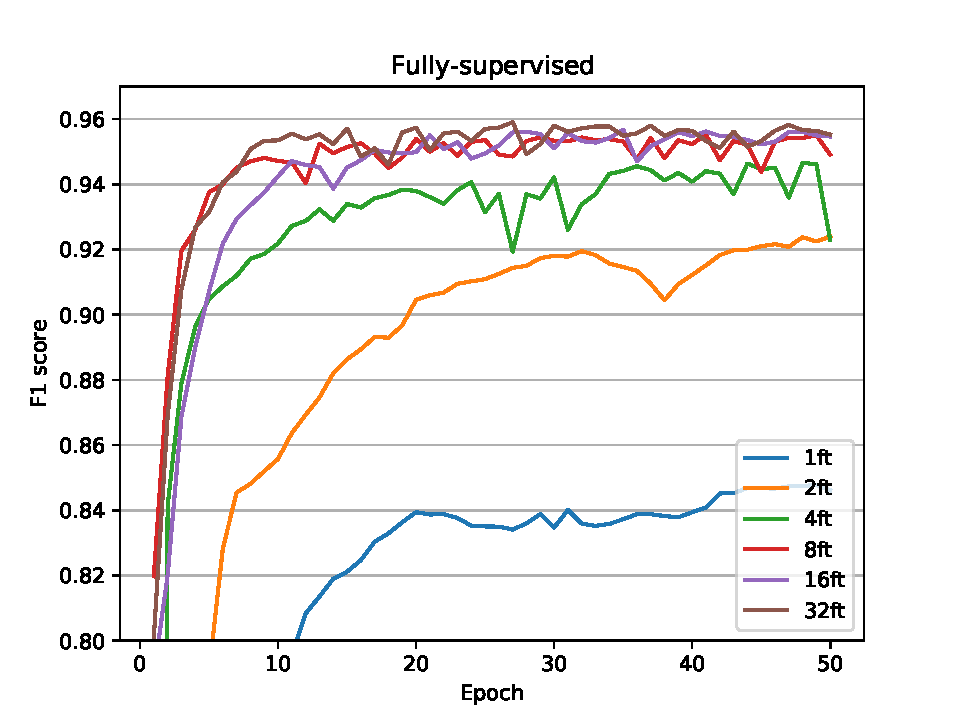
\includegraphics[width=140mm]{../../figures/02-cvc-improvements/supervised.pdf}
    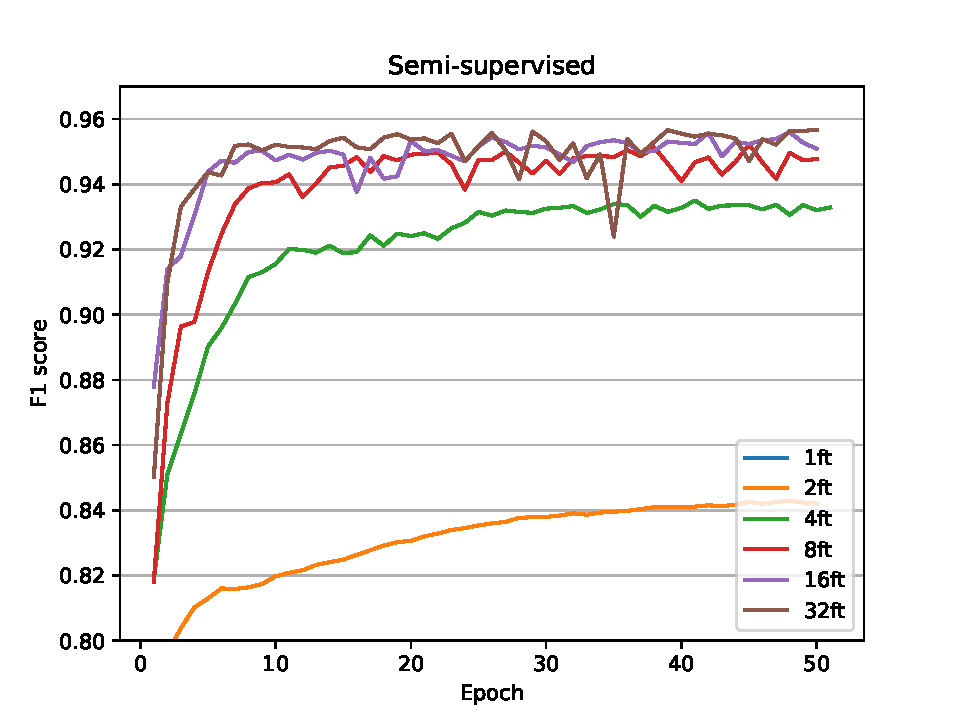
\includegraphics[width=140mm]{../../figures/02-cvc-improvements/semisupervised.pdf}
    \caption{Comparison of fully-supervised and semi-supervised training regimes with models of varying capacity (inner feateures) on the CVC-MUSCIMA dataset. Both regimes get to the same performance, below the 96\% line. The model 1 in semi-supervised regime peaks below 80\% line and is not visible in the chart.}
    \label{fig:CvcImprovements}
\end{figure}

Since the dataset is now much larger than in the previous experiment (section \ref{sec:SemisupervisedImprovements}), we no longer need dropout layers. In fact, the training is even more stable without it and individual runs are clearly separated.

This experiment attempts to compare fully-supervised and semi-supervised models regardless of their capacity. We therefore train various model capacities (the \emph{inner features} model parameter) and then compare the best ones for each setting.

Another difference to the previous experiment is that the ratio of labeled to unlabeled data is fixed and given by dataset sizes. The ratio of 99 to 551 pages corresponds best with the ratio 10:50.

The validation dataset F1 score over the course of training can be seen in figure \ref{fig:CvcImprovements}. In these charts we can see:

\begin{itemize}
    \item Models with 1 and 2 \emph{inner features} are clearly underfitting in the supervised mode (compared to other models). When we add unlabeled data, their perfomance drops significantly, but the training curve gets much smoother.
    \item Models with 4 and 8 \emph{inner features} worsen much less and also get smoother (especially 4 becomes much more stable).
    \item Model 16 no longer worsens, it is able to learn both tasks.
\end{itemize}

Conclusions can be drawn from these observations:

\begin{itemize}
    \item The reconstruction and segmentation tasks clearly compete for model capacity. The performance drop due to adding unlabeled data decreases, as the model capacity increases.
    \item The addition of unlabeled data can be used as a regularization technique. This is evident from the fact that training curves get much smoother as we add unlabeled data (especially for models 2 and 4). A~regularization effect is also described in the corresponding literature (\cite{SemisupervisedOverview}).
    \item All models come close to the 96\% line, but never cross it. While the semi-supervised models get as good as the fully-supervised, they never get better. It seems the reconstruction task is not learning any useful representations. But from section \ref{sec:NoiseParameters} we know that some abstract representations are learned. Maybe these learned representations are not used during segmentation.
\end{itemize}


\section{Knowledge Transfer}
\label{sec:KnowledgeTransfer}

The goal of this experiment is to train a model to transfer a learned task from one domain onto another in a semi-supervised manner. The goal is to perform semantic segmentation on handwritten music, while providing labels only for printed music. We use the DeepScores v2 dataset (\cite{DeepScores}) as the source of labeled printed music and the MUSCIMA++ dataset (\cite{MuscimaPP}) as the source of unlabeled handwritten music. Validation is performed on a set of 20 pages from the MUSCIMA++ dataset. We use the remaining 99 pages for unsupervised training. To keep the ratio of labeled to unlabeled data at a reasonable value of 1:5, we use 20 labeled pages from the DeepScores dataset. We also train a supervised baseline with no unlabeled pages to compare against.

We first tried performing notehead segmentation, like in the previous experiments, but the results were extremely noisy and no meaningful difference could be seen. The pixelwise F1 score varied from 0.2 to 0.6 even between different runs of the supervised baseline (with dataset seed fixed). Semi-supervised runs were equally noisy and within the same range. When inspecting the infered segmentation masks, we concluded that handwritten noteheads are overly varied and have very different appearance compared to printed noteheads. The trained models could only reliably segment noteheads of writer 9, whose noteheads are very similar to printed ones.

Informed by this failure, we choose to segment stafflines. Firstly, because they are very easy geometric shapes to understand. Stafflines are the first objects that a model learns to repair during reconstruction and does so with great precision. Secondly, thier visual appearance in the printed and handwritten datasets is very similar, but not identical. A challenge is still being presented (handwritten stafflines are much thinner and the surrounding symbols are more varied).

We set model capacity to 8 \emph{inner features} and train for 20 epochs. The training process is still relatively noisy (like the failed notehead attempts), so we train both the supervised and semi-supervised variants 4 times each and compute an average. Results can be seen in figure \ref{fig:StafflineTransfer}.

\begin{figure}[ht]
    \centering
    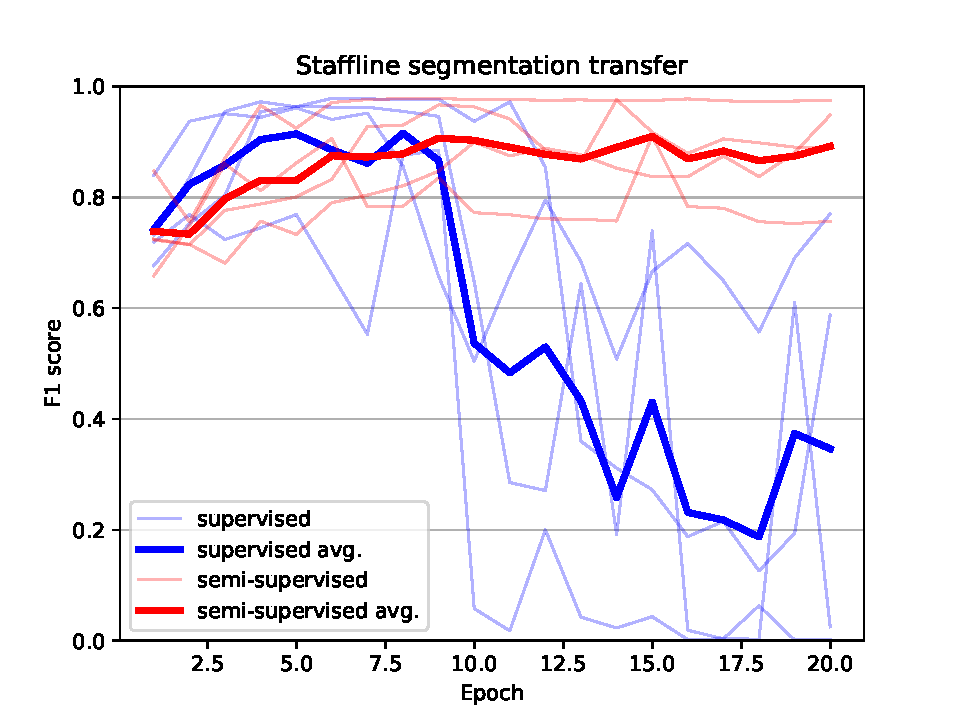
\includegraphics[width=140mm]{../../figures/04-staffline-transfer/transfer.pdf}
    \caption{Handwritten staffline segmentation F1 score, when training on labeled printed music and unlabeled handwritten music.}
    \label{fig:StafflineTransfer}
\end{figure}

During the first 7 epochs, both variants perform equally well, however at about the tenth epoch all fully-supervised models start overfitting and their F1 score drops to very low numbers. Interestingly, all the semi-supervised models stay at a comparably high score. They seem to plateau, instead of overfitting. This is a clear example of how the unsupervised data can regularize the training and prevent the model from overfitting. Unfortunately, if we take the best checkpoints of both variants, we see that both variants perform equally well. The semi-supervised model does not surpass the supervised baseline.

\begin{figure}[ht]
    \centering
    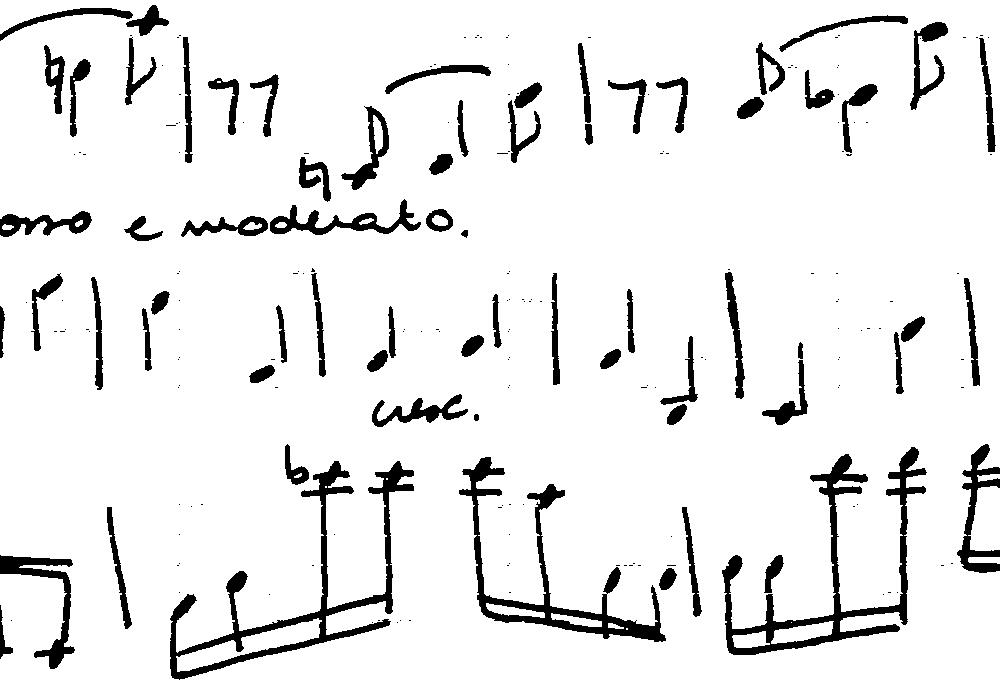
\includegraphics[width=140mm]{../../figures/04-staffline-transfer/staffline-removal.png}
    \caption{Handwritten stafflines removed by the model trained on labeled printed music and unlabeled handwritten music. Tiny speckles in the image are the result of imperfect segmentation.}
    \label{fig:StafflineRemoval}
\end{figure}

Evaluating the best semi-supervised model on the MUSCIMA++ test set (writer-independent) gives us a pixelwise F1 score of 97.70\%. The same model peaks on the validation set at 97.81\%. 

We can compare ourselves to an article by \cite{StafflineDetection}, focusing on staffline removal. The article presents a convolutional network trained in a supervised way on a dataset extracted from the CVC-MUSCIMA dataset (\cite{CvcMuscima}). The table 4 in the article provides their pixelwise F1 score on undistorted images (99.25\%) together with other older approaches (97.59\% up to 98.51\%). We can see that our results are in a range comparable to older approaches, which is impressive, since we did not use a single annotated handwritten image. Our annotated training images were purely digitally constructed, without any attempts at mimicking the handwritten style.

